%=======================================================================
%  Grutas de Aroe-Jari — artigo em grupo
%  CPS837 Projeto de Jogos · PESC/COPPE/UFRJ · 2026/2
%
%  Compilar:  latexmk -pdf artigo.tex
%       ou:   pdflatex artigo && bibtex artigo && pdflatex artigo && pdflatex artigo
%=======================================================================
\documentclass[conference]{IEEEtran}

\usepackage[utf8]{inputenc}
\usepackage[T1]{fontenc}
\usepackage[brazilian]{babel}
\usepackage{cite}
\usepackage{graphicx}
\usepackage{booktabs}
\usepackage{array}
\usepackage{amsmath}
\usepackage{xcolor}
\usepackage{url}
\usepackage[hidelinks]{hyperref}

\graphicspath{{figuras/}}

% Marcador visível para o que ainda falta preencher com dados reais.
\newcommand{\preencher}[1]{\textcolor{red}{\textbf{[PREENCHER: #1]}}}

\begin{document}

\title{Do mito à mecânica: projeto, desenvolvimento e\\
avaliação preliminar de \textit{Grutas de Aroe-Jari},\\
um jogo digital sobre uma narrativa do povo Boé (Bororo)}

\author{%
\IEEEauthorblockN{Maximilian Sabino Ribeiro}
\IEEEauthorblockA{Programa de Engenharia de Sistemas e Computação\\
COPPE, Universidade Federal do Rio de Janeiro\\
Email: mribeiro@cos.ufrj.br}
\and
\IEEEauthorblockN{Breno G. de Oliveira}
\IEEEauthorblockA{Programa de Engenharia de Sistemas e Computação\\
COPPE, Universidade Federal do Rio de Janeiro\\
Email: breno@cos.ufrj.br} }

\maketitle
\bstctlcite{IEEEctl}

%=======================================================================
\begin{abstract}
A revisão sistemática mais recente sobre patrimônio cultural em jogos digitais aponta que
o patrimônio material domina a literatura enquanto o imaterial (rito, narrativa oral, significado simbólico) permanece sub-representado. Este artigo relata o projeto, o
desenvolvimento e a avaliação preliminar de \textit{Grutas de Aroe-Jari}, jogo digital 2D
de vista superior construído em Godot~4 sobre uma narrativa atribuída ao povo Boé
(Bororo), em que o herói Pari Jura prepara uma armadilha para a serpente Butoriko. O
trabalho segue Design Science Research e articula a tradução do mito em mecânica, o relato
de desenvolvimento e a ética da representação. O protótipo reúne 3.851 linhas de
GDScript, 16 cenas, uma gruta de 636 células, 13 itens distintos em 44 instâncias e 11
pinturas rupestres, dez das quais ensinam receitas de combinação, feitos por dois
desenvolvedores em doze dias e 57 \textit{commits}.
Três resultados principais são reportados. Uma matriz de correspondência mostra que a
matéria do mito sobreviveu à implementação, mas não a sua estrutura: o laço de extração
ficou de fora. A comparação entre design e artefato localiza o encolhimento de escopo nos
sistemas que atravessam fronteiras de cena. E a busca por um registro publicado da
narrativa, que a tradição Boé transmite mas que nenhum acervo digitalizado permitiu citar,
sustenta uma discussão sobre o descompasso entre tradição e registro citável. Discute-se ainda o risco de
reinscrever a lógica extrativista sobre uma cosmologia indígena e propõe-se um quadro de
decisão rastreável.
\end{abstract}

\begin{IEEEkeywords}
jogos digitais, patrimônio cultural imaterial, povos indígenas, povo Boé (Bororo),
Godot Engine, Design Science Research, relato de desenvolvimento.
\end{IEEEkeywords}

%=======================================================================
\section{Introdução}
\label{sec:introducao}

Há uma assimetria bem documentada na pesquisa sobre jogos e patrimônio cultural.
Revisando oitenta publicações, Que, De La Hera e Jansz~\cite{que2025} concluem que o
patrimônio \textit{material} (arquitetura, artefato, sítio) concentra a atenção da área,
enquanto o patrimônio \textit{imaterial} (rito, narrativa oral, significado simbólico)
aparece com frequência bem menor; e observam, no mesmo movimento, que a produção se
concentra num repertório estreito de gêneros. Costa \textit{et al.}~\cite{costa2025},
revisando vinte anos de \textit{cultural game-making} com jovens, acrescentam um segundo
diagnóstico: quando a comunidade detentora do saber aparece, aparece enquadrada como
aprendiz, quase nunca como cocriadora.

Este artigo relata um projeto que se situa exatamente nesse ponto cego e que, por isso
mesmo, esbarra em todos os seus problemas. \textit{Grutas de Aroe-Jari} é um jogo
digital 2D de vista superior, desenvolvido em Godot~4 no contexto da disciplina CPS837
(Projeto de Jogos), do Programa de Engenharia de Sistemas e Computação da COPPE/UFRJ.
Seu material de partida é uma narrativa atribuída ao povo Boé, nome pelo qual se
autodesigna o povo conhecido na literatura como Bororo~\cite{serpa2025}. Nela, o moço
Pari Jura, depois de a mãe ser devorada pela serpente Butoriko, prepara uma sequência de
obstáculos no caminho de fuga, desperta o monstro e o mata quando ele fica preso sob um
cerne de sucupira. O jogador assume o papel de Pari Jura, entra na gruta de Aroe-Jari
com uma tocha que se consome, coleta matéria-prima entre as ossadas das vítimas e monta
as armadilhas com que enfrentará a serpente.

O objetivo geral do trabalho é projetar, construir e avaliar preliminarmente esse
artefato, tratando-o como objeto de conhecimento e não apenas como entrega de
disciplina. Como objetivos específicos: (i)~documentar a tradução do material narrativo
em mecânica de jogo, elemento a elemento, de modo que a correspondência possa ser
auditada por terceiros; (ii)~comparar sistematicamente o documento de design com o
artefato efetivamente entregue, localizando onde o escopo encolheu e por quê;
(iii)~separar o que vem da tradição do que é adaptação nossa, e relatar a busca pela
referência documental da narrativa; e (iv)~propor um quadro de decisão
rastreável para projetos que, como este, operam em posição consultiva e não em regime de
codesenvolvimento com a comunidade detentora do saber.

A contribuição que reivindicamos é dupla e deliberadamente modesta. A primeira é
metodológica: separamos, elemento a elemento, o que o projeto recebeu da tradição Boé do
que ele inventou para transformá-la em jogo, e relatamos a busca, malsucedida, por um
registro publicado dessa narrativa. Desse relato extraímos um problema que nos parece
geral: a pesquisa em patrimônio imaterial trabalha com material que pode ser inteiramente
real e ainda assim inteiramente incitável, porque é oral, ou está em acervos que a
digitalização não alcançou. A segunda
contribuição é analítica: mostramos que a mecânica que melhor traduziria a estrutura do
mito, o laço de extração (isto é, a decisão de quando parar de acumular e sair), foi
projetada, foi parcialmente codificada e, ainda assim, não chegou ao protótipo, e que
essa ausência é explicável por uma característica estrutural do cronograma, não por
falta de ideia.

O restante do artigo se organiza como segue. A Seção~\ref{sec:referencial} apresenta o
referencial teórico e os trabalhos relacionados. A Seção~\ref{sec:metodo} descreve a
metodologia, o contexto de produção e, com o detalhe que o caso exige, a origem da
narrativa e o problema da sua referência. A Seção~\ref{sec:artefato} descreve o artefato. A
Seção~\ref{sec:resultados} apresenta os resultados. A Seção~\ref{sec:discussao} os
interpreta frente à literatura. A Seção~\ref{sec:conclusao} conclui.

%=======================================================================
\section{Referencial Teórico e Trabalhos Relacionados}
\label{sec:referencial}

\subsection{Representação de povos indígenas em jogos digitais}

O campo tem em Elizabeth LaPensée sua referência mais articulada. Em
\textit{Self-Determination in Indigenous Games}~\cite{lapensee2018}, ela argumenta que o
jogo digital é um meio particularmente potente para a expressão indígena justamente
porque estratifica regra, história, arte e som, e que o critério de avaliação não pode
ser a fidelidade da representação, mas o grau de autodeterminação exercido na produção.
O conceito é depois formalizado por LaPensée, Laiti e Longboat~\cite{lapensee2022} como
\textit{jogo soberano}: aquele em que o povo indígena mantém autonomia decisória em
todas as fases, da concepção à distribuição. Trata-se de um critério normativo, não
descritivo: permite dizer onde um projeto está, e não apenas se ele é bem-intencionado.

O relato de \textit{When Rivers Were Trails}~\cite{lapensee2021} é o precedente
metodológico mais próximo do nosso caso: um jogo 2D de aventura escrito por autores
indígenas, com análise explícita do processo. Emmons e LaPensée~\cite{emmons2021}
avaliam empiricamente sua recepção por estudantes indígenas, oferecendo um modelo de
seção de avaliação. Madsen~\cite{madsen2017}, analisando
\textit{Never Alone} e \textit{Invaders}, desloca a discussão da representação para as
\textit{mecânicas}, mostrando como a \textit{survivance} se inscreve nas regras e não
apenas na superfície audiovisual. Esse deslocamento é o eixo teórico central deste
artigo. Nijdam~\cite{nijdam2023a,nijdam2023b} o confirma no corpus Sámi, e
Laiti~\cite{laiti2025} conecta o design de jogos indígenas aos princípios de governança
de dados indígenas. Byrd~\cite{byrd2025} radicaliza a crítica: a estrutura da
desapropriação colonial estaria codificada nas próprias mecânicas dos jogos comerciais
(expansão como progresso, território como recurso), de modo que a superfície
``respeitosa'' pode conviver com uma gramática colonial intacta.
Wallis~\cite{wallis2023} documenta a variante mais corriqueira do problema: estética
indígena sem povos indígenas.

No Brasil, o precedente decisivo é Meneses~\cite{meneses2017}, sobre a criação de
\textit{Huni Kuin: Yube Baitana} com o povo Huni Kuin, que enfrenta de frente a questão da
circulação de saberes, do direito autoral e dos acordos etnográficos. Martins Neto
\textit{et al.}~\cite{martinsneto2024} propõem, no SBGames, uma agenda de
``representação responsável'' e organizam os casos brasileiros exemplares. Somam-se
relatos de processo como \textit{Menoari}~\cite{moraes2023}, o jogo educativo de apontar
e clicar de Garone \textit{et al.}~\cite{garone2023} e, mais recentemente,
\textit{Entre Lendas e Pixels}~\cite{locatelli2025}, sobre patrimônio imaterial alagoano, o trabalho brasileiro mais próximo do nosso em escopo e gênero.

\subsection{Ética da representação e governança de saberes}

Os princípios CARE para governança de dados indígenas~\cite{carroll2020} são o arcabouço
normativo mais citado (benefício coletivo, autoridade de controle, responsabilidade e
ética), formulados como complemento aos princípios FAIR justamente porque abertura sem
autoridade de controle reproduz espoliação. No plano jurídico brasileiro, a
Convenção~169 da OIT~\cite{oit1989} estabelece o direito à consulta livre, prévia e
informada, e a Lei~11.645/2008~\cite{brasil2008} torna obrigatório o ensino de história
e cultura indígena na educação básica, o que constitui, de passagem, o principal
argumento de utilidade pública para jogos como o descrito aqui. A Convenção da UNESCO de
2003~\cite{unesco2003} fornece a definição operante de patrimônio cultural imaterial.

Vasalou \textit{et al.}~\cite{vasalou2014} problematizam a apropriação cultural do ponto
de vista do design de interação, deslocando o critério do produto para o processo.
Arrivabene~\cite{arrivabene2025} leva o argumento adiante em chave decolonial: os
métodos correntes de game design carregariam pressupostos coloniais (expansão, acúmulo,
extração de recursos) que sobrevivem intactos a qualquer troca de temática. É a objeção
mais séria que se pode fazer ao projeto aqui descrito, e nós a retomamos na
Seção~\ref{sec:discussao}.

\subsection{Jogos sérios e patrimônio cultural imaterial}

Além da revisão de Que \textit{et al.}~\cite{que2025} já citada, três trabalhos recentes
sustentam o desenho deste artigo. Camuñas-García \textit{et al.}~\cite{camunas2023}
propõem um quadro de avaliação de jogos de patrimônio em três dimensões (cognitiva,
emocional e comportamental) que adotamos como instrumento na Seção~\ref{sec:resultados}.
Roy \textit{et al.}~\cite{roy2024} tratam especificamente da gamificação de expressões
\textit{orais} de patrimônio têxtil indígena, o paralelo internacional mais próximo do
nosso objeto. Laiti \textit{et al.}~\cite{laiti2021} mostram, no caso do Sámi Game Jam,
que o próprio evento de criação pode operar como prática de sustentação de patrimônio
imaterial. No Brasil, Moura
\textit{et al.}~\cite{moura2025} oferecem o modelo de artigo ``jogo étnico-educacional
com avaliação'', e Hoffmann e Paschke~\cite{hoffmann2025} propõem o rótulo
\textit{anthrogames} para jogos que veiculam conhecimento antropológico, admitindo que
faltam ao campo quadros de avaliação de representação cultural.

Dois desses trabalhos merecem comparação direta, porque são os precedentes mais
próximos. Roy \textit{et al.}~\cite{roy2024} partem, como nós, de expressão oral e não
de sítio ou artefato, mas resolvem, pela coleta em campo, o
problema que nos ficou aberto: trabalham com depoimentos recolhidos junto às comunidades
têxteis do nordeste indiano, o que lhes dá referência rastreável para cada expressão
gamificada, enquanto nós usamos material da tradição sem conseguir localizar um registro
que o cite. \textit{Entre Lendas e
Pixels}~\cite{locatelli2025} é o mais próximo em escopo, gênero e contexto de produção
(jogo digital brasileiro sobre patrimônio imaterial regional, em equipe acadêmica), e a
diferença de desenho está no que cada projeto faz com a narrativa: lá, o folclore
alagoano é apresentado ao jogador como conteúdo a conhecer; aqui, tentamos inscrevê-lo
na regra. A Seção~\ref{sec:resultados} mostra até onde essa tentativa chegou.

\subsection{Do conteúdo à mecânica}

A tradição de design que sustenta a operação central deste trabalho é conhecida.
Jenkins~\cite{jenkins2004} descreve o design de jogos como arquitetura narrativa, em que
a história é distribuída pelo espaço e recuperada pela exploração, em vez de narrada em
cenas; é o que justifica contar o mito pelo desenho da gruta e pelas pinturas de parede,
e não por cinemáticas. Bogost~\cite{bogost2007} formula a retórica procedural: o
argumento que um jogo faz está no que suas regras permitem, obrigam e proíbem. Do modelo
MDA~\cite{hunicke2004} tomamos apenas a separação entre a regra e o que ela produz na
experiência, que sustenta o par matéria/estrutura da Seção~\ref{sec:resultados}; Salen e
Zimmerman~\cite{salen2003} e Schell~\cite{schell2019} fornecem o instrumental de
projeto. No enquadramento local, o relatório do LUDES~\cite{xexeo2017jogos} sustenta a
definição de jogo adotada e o método \textit{Play Your Process}~\cite{classe2019play}
oferece o precedente institucional de derivar mecânica de uma estrutura externa ao jogo:
ali, um processo de negócio; aqui, uma narrativa.

\subsection{O laço de extração e a economia do risco}

O gênero que o projeto mobiliza, comumente chamado de \textit{extraction shooter} ou, na
formulação do nosso documento de design, \textit{roguelite de armadilha e fuga}, carece
de literatura acadêmica revisada por pares, apesar de sua penetração comercial. O que
existe, e que usamos, é o instrumental adjacente. Cartlidge~\cite{cartlidge2024}
argumenta que gêneros como o \textit{roguelike} devem ser definidos pela experiência que
produzem (avaliação contínua de ameaça em cenário tático) e não por listas de mecânicas,
o que nos autoriza a caracterizar o laço de extração pela decisão que ele força. Tomé
\textit{et al.}~\cite{tome2020} demonstram experimentalmente que a aversão à perda opera
dentro do círculo mágico~\cite{huizinga2000}, com jogadores exigindo ganhos superiores
ao dobro da perda potencial para aceitar risco. West \textit{et al.}~\cite{west2022}
mostram que a morte permanente aumenta a apreciação do jogo, mediada pelo luto;
Parker~\cite{parker2017} liga o fenômeno à Terror Management Theory; e
Toh~\cite{toh2021} mapeia os quadros de decisão econômica que o jogador mobiliza.
Sweetser e Wyeth~\cite{sweetser2005} fornecem o modelo GameFlow, alternativa ao
instrumento adotado na Seção~\ref{sec:playtest} e candidato para a avaliação com
usuários indicada na Seção~\ref{sec:conclusao}.

\subsection{Godot Engine e desenvolvimento acadêmico}

Holfeld~\cite{holfeld2024} mede empiricamente a relevância da Godot no mercado
independente; Peña Pérez Negrón \textit{et al.}~\cite{penaperez2023} a apresentam como
plataforma didática; Guerreiro \textit{et al.}~\cite{guerreiro2021} relatam
desenvolvimento 2D em Godot em contexto acadêmico brasileiro, justificando a escolha por
GDScript, licença permissiva e custo zero, as mesmas razões que nos levaram a ela.
Öztürk~\cite{ozturk2025} oferece o contraponto necessário, classificando a Godot como de
manutenibilidade comparativamente baixa em análise estática, apesar de sua posição de
mercado.

\subsection{O povo Boé (Bororo)}

Os Boé habitam o cerrado e a borda do Pantanal em Mato Grosso, em terras indígenas como
Meruri, Sangradouro, Tadarimana, Perigara, Teresa Cristina e Jarudori; o território
atual é uma fração do território tradicional documentado por
Costa~\cite{costaikuiapa2019}, que ia do rio Otuquis às bacias do Paraguai, do
Cuiabá-São Lourenço e do Araguaia~\cite{serpa2025}. O corpus etnográfico é denso: a base
salesiana da
\textit{Enciclopédia Bororo}~\cite{albisetti1962,albisetti1969}, o trabalho fundador de
Lévi-Strauss~\cite{levistrauss1936}, a etnografia de Crocker~\cite{crocker1985} e os
estudos de Viertler~\cite{viertler1991} e Novaes~\cite{novaes2006} sobre o funeral.

Dois conceitos importam diretamente ao jogo. O primeiro é \textit{aroe}: a alma, o
espírito do morto e do ancestral clânico, contraposto ao \textit{bope}, potência de
transformação associada ao nascimento, à putrefação e à morte~\cite{serpa2025}. O
topônimo da caverna que dá nome ao jogo (Aroe Jari, na Chapada dos Guimarães, a maior
caverna em arenito do Brasil) é regularmente glosado como morada das almas, leitura
coerente com a associação entre \textit{aroe} e o destino dos mortos descrita na
etnografia~\cite{crocker1985,viertler1991}. O segundo é \textit{bakaru}.
Souza~\cite{souzabakaru,souza2014}, em etnografia na Aldeia Central de Tadarimana,
registra que os próprios Boé traduzem \textit{bakaru} não como ``lenda'', mas
simultaneamente como história do povo, fundamento da vida e código de conduta: o
\textit{bakaru} orienta a divisão das metades exogâmicas Tugarege e Ecerae, as uniões
matrimoniais, as restrições alimentares e o cuidado com os mortos. Um interlocutor da
pesquisa resume: ``Bakaru é o local onde estão os códigos de conduta do Bororo. Bororo
que perdeu de vista o bakaru não vive mais como Bororo''~\cite{souzabakaru}.

Essa definição tem consequência direta para o nosso projeto e a registramos aqui porque
ela reorganiza o problema: tratar um \textit{bakaru} como enredo de jogo é tratar como
matéria-prima ficcional aquilo que, para a comunidade de origem, é norma. O trabalho de
Ekureu~\cite{ekureu2025}, professor Boé da Escola Indígena de Meruri, escrevendo em
primeira pessoa sobre o \textit{pariko}, o diadema de penas em que se inscrevem as
insígnias clânicas, torna o ponto ainda mais concreto: há elementos da cultura Boé cujo
uso é regulado internamente por clã, por metade e por momento cerimonial, e cuja
exibição fora de contexto não é neutra. Souza \textit{et al.}~\cite{souzaboe2025}, em
trabalho com coautoria indígena, e Isaac e Pereira Junior~\cite{isaac2021} discutem
precisamente a tensão entre esses saberes e a escolarização.

\subsection{Posicionamento}

O presente trabalho não é um jogo soberano no sentido de LaPensée
\textit{et al.}~\cite{lapensee2022}, nem um codesenvolvimento no sentido de
Meneses~\cite{meneses2017}. É um exercício acadêmico de dois desenvolvedores não
indígenas, sem consulta à comunidade, produzido em doze dias. Dizer isso aqui, no
referencial, e não numa nota final de limitações, é uma escolha deliberada: é a condição
para que o restante do artigo, inclusive o que ele reivindica como contribuição, possa
ser lido pelo que é.

%=======================================================================
\section{Metodologia}
\label{sec:metodo}

\subsection{Design Science Research como estrutura}

O trabalho segue Design Science Research~\cite{hevner2004,peffers2007}: o objeto de
estudo é um artefato construído, e o conhecimento se produz no ciclo entre projetá-lo,
avaliá-lo e revisá-lo à luz do que a avaliação mostra. Percorremos as seis etapas de
Peffers \textit{et al.}~\cite{peffers2007} da seguinte forma: identificação do problema
(a lacuna de patrimônio imaterial apontada por Que \textit{et al.}~\cite{que2025});
definição de objetivos (traduzir uma narrativa oral em mecânica, e não em cenário);
projeto e desenvolvimento (o SGDD~\cite{sgdd2026} e o protótipo em
Godot~\cite{repo2026}); demonstração (a \textit{build} jogável para Windows e
navegador); avaliação (as três frentes da Seção~\ref{sec:resultados}); e comunicação
(este artigo).

Sobre essa estrutura enxertamos a técnica de coleta consolidada na literatura de
engenharia de software para jogos: o relato pós-projeto sistemático. Petrillo
\textit{et al.}~\cite{petrillo2009} inauguraram a linha ao levantar problemas
recorrentes em relatos publicados; Washburn \textit{et al.}~\cite{washburn2016}
analisaram 155 \textit{post-mortems}; e Politowski
\textit{et al.}~\cite{politowski2021} estenderam a análise à literatura cinzenta,
concluindo que as causas-raiz dos problemas de desenvolvimento são predominantemente
humanas e de processo, não técnicas. Calhabeu e Lima~\cite{calhabeu2025} e Xexéo
\textit{et al.}~\cite{xexeo2026enigma} fornecem o precedente recente de relato de
experiência em contexto acadêmico como artigo completo.

\subsection{Contexto, equipe e restrições}

O projeto foi desenvolvido na disciplina CPS837 (Projeto de Jogos), do PESC/COPPE/UFRJ,
no período 2026/2. A equipe é de duas pessoas, ambas com experiência prévia em
programação e nenhuma com formação em antropologia. Não houve orçamento, contratação de
arte ou consultoria. A janela efetiva de desenvolvimento foi de doze dias corridos,
entre 24 de julho e 4 de agosto de 2026, concorrendo com as demais obrigações do
semestre. Essas restrições não são desculpa: são o objeto. Elas descrevem a situação
típica em que jogos brasileiros de temática cultural são produzidos em contexto
acadêmico, e a análise de escopo da Seção~\ref{sec:resultados} só faz sentido à luz
delas.

A escolha da Godot~4~\cite{godot2026} seguiu os critérios já relatados por Guerreiro
\textit{et al.}~\cite{guerreiro2021}: licença permissiva, custo zero, exportação para
navegador em um passo e GDScript com curva de entrada curta. Adotou-se o \textit{preset}
de compatibilidade OpenGL para maximizar a chance de a \textit{build} web rodar em
máquinas de terceiros.

\subsection{A narrativa de base e o que dela é nosso}
\label{sec:procedencia}

Esta subseção separa duas coisas que o restante do artigo precisa manter separadas: o que
o projeto recebeu da tradição Boé e o que o projeto inventou. Sem essa linha, nem o
crédito nem a responsabilidade caem no lugar certo.

\textbf{A narrativa é da tradição Boé.} A história de Pari Jura, que perde a mãe para a
serpente Butoriko, prepara o caminho de fuga com uma sequência de obstáculos e a mata
quando ela fica presa sob o cerne de sucupira, chegou ao projeto como narrativa do povo
Boé, e é assim que a tratamos. Nada nela foi inventado por nós.

\textbf{A adaptação é nossa.} A gruta como labirinto navegável, a tocha que se consome e
define o campo de visão, o catálogo de itens e as receitas de combinação, as armadilhas
como objetos que o jogador planta no chão, a perda parcial de carga na morte e o
enfrentamento organizado como partida são invenções do projeto, feitas para converter uma
narrativa em algo jogável. A Tabela~\ref{tab:mito} detalha essa conversão elemento a
elemento. Onde o jogo se afasta da história, a responsabilidade é nossa.

Três leituras orientaram o tratamento do material, e vale explicitar o que cada uma
decidiu. Souza~\cite{souzabakaru,souza2014}, em etnografia na Aldeia Central de
Tadarimana, mostra que \textit{bakaru} não traduz ``lenda'': os próprios Boé o descrevem
simultaneamente como história do povo, fundamento da vida e código de conduta. Isso
reposiciona o que significa usar uma dessas narrativas como matéria de jogo, e é a razão
de o artigo não tratar o material como folclore disponível.
Ekureu~\cite{ekureu2025}, professor Boé da Escola Indígena de Meruri escrevendo em
primeira pessoa sobre o \textit{pariko}, o diadema de penas em que se inscrevem as
insígnias clânicas, mostra que há elementos cuja confecção, uso e exibição são regulados
por clã, por metade e por momento cerimonial. Foi essa leitura que nos levou a manter fora
do jogo qualquer grafismo clânico e qualquer elemento cerimonial. E a associação entre
\textit{aroe} e o destino dos mortos~\cite{serpa2025,crocker1985} é o que dá sentido ao
topônimo da gruta e à decisão de povoá-la de ossadas.

\subsection{A referência que não conseguimos estabelecer}
\label{sec:referencia}

Para citar a narrativa como manda a prática acadêmica, precisaríamos de um registro
publicado. Não o encontramos, e o relato dessa busca é parte dos resultados deste
trabalho.

Buscamos, em agosto de 2026, em português, espanhol e inglês, as grafias
\textit{Pari Jura}, \textit{Pariogo}, \textit{Pari Jurá}, \textit{Butoriko} e
\textit{Botoriko}, cruzadas com os termos \textit{sucuri}, \textit{serpente},
\textit{coroatá}, \textit{cipó unha-de-gato}, \textit{urubamba}, \textit{sucupira} e
\textit{Aroe Jari}, em repositórios de teses brasileiros, no acervo digital da FUNAI, na
base do Instituto Socioambiental e na literatura secundária sobre a \textit{Enciclopédia
Bororo}~\cite{albisetti1969}. \emph{Nenhum registro publicado foi localizado.} A narrativa
também não corresponde ao \textit{bakaru} mais difundido, a Grande Inundação de Meriri
Poro, nem ao mito do desaninhador de pássaros que Lévi-Strauss tomou como referência
inaugural das \textit{Mitológicas}~\cite{levistrauss1964}.

O que esse resultado significa precisa ser dito com cuidado, porque a leitura apressada
seria exatamente a errada. Ele \textbf{não} indica que a narrativa não pertença à tradição
Boé. Indica que o acervo em que ela estaria registrada não é acessível por busca digital.
O volume~II da \textit{Enciclopédia Bororo}~\cite{albisetti1969}, que, segundo
Souza~\cite{souzabakaru}, reúne 62 \textit{bakaru} agrupados em sete categorias, não está
disponível em texto integral \textit{online}. E, antes disso, uma tradição oral não se
esgota no que foi publicado: a ausência de registro é um fato sobre os arquivos, não sobre
a tradição.

Enquanto a referência não for estabelecida, este artigo cita a narrativa como pertencente
à tradição Boé, sem atribuí-la a autor ou obra específica, e registra a conferência
documental do volume~II como pendência na Seção~\ref{sec:conclusao}. A mesma declaração
acompanha o repositório do projeto e a tela de contexto do jogo.

O ponto que nos parece generalizável é o descompasso entre \textbf{tradição e registro
citável}. A pesquisa em patrimônio imaterial trabalha com material que pode ser
inteiramente real e ainda assim inteiramente incitável, porque o que existe é oral, ou
está em acervos que a digitalização não alcançou. Uma equipe pequena, com prazo curto e
sem acesso a biblioteca especializada, encontra então uma escolha ruim: abandonar o
material, ou usá-lo sem poder referenciá-lo. Nenhuma das duas é boa, e a segunda é a que
se pratica em silêncio. A saída que adotamos é declarar a cadeia inteira, o que recebemos,
o que buscamos, o que não achamos e o que falta conferir, de modo que o leitor possa julgar
o material pelo que ele é. Diante do CARE, isso toca a dimensão de \textit{autoridade de
controle}~\cite{carroll2020} por um ângulo pouco discutido: a comunidade não pode exercer
autoridade sobre o uso de um saber que o meio acadêmico sequer consegue nomear com
precisão.

\subsection{Instrumentos de coleta}

Três fontes de dados sustentam a Seção~\ref{sec:resultados}.

\textbf{O repositório.} Todas as métricas de artefato e de processo foram extraídas
programaticamente do repositório Git do projeto~\cite{repo2026}: contagem e autoria de
\textit{commits}, linhas de GDScript por script, cenas, contagem e posição de cada
entidade instanciada na cena da caverna, e a geometria de colisão do \textit{tileset},
esta última decodificada diretamente do \texttt{PackedByteArray} da camada de
\textit{tilemap}, o que permitiu reconstruir a planta da gruta apresentada na
Fig.~\ref{fig:planta} sem depender de captura de tela.

\textbf{Os documentos de design.} Duas versões do SGDD~\cite{sgdd2026} foram
preservadas: uma descrição textual corrida com listas de tarefas de arte, programação,
áudio e interface, e uma versão posterior em folha única no formato consolidado por
Rogers~\cite{rogers2014}. A comparação entre a segunda versão e o artefato final produz
a Tabela~\ref{tab:gap}.

\textbf{O teste com jogadores.} Uma sessão informal de teste foi conduzida ao fim do
período de desenvolvimento. O protocolo e os achados são reportados na
Seção~\ref{sec:playtest}, com o instrumento de Camuñas-García
\textit{et al.}~\cite{camunas2023} como grade de análise.

\subsection{Ameaças à validade}

Quatro ameaças precisam ser declaradas antes dos resultados. \textit{Validade de
construto}: as métricas de repositório medem atividade e volume, não qualidade; um
\textit{commit} não é uma unidade de trabalho comparável a outro. \textit{Validade
interna}: os dois autores deste artigo são os dois desenvolvedores do jogo, de modo que
a análise de escopo é autorrelato, sujeito a racionalização retrospectiva, risco que
mitigamos ancorando cada afirmação em evidência extraível do repositório.
\textit{Validade externa}: um projeto de doze dias e duas pessoas não generaliza para
produção comercial. \textit{Validade de conclusão}: o teste com jogadores é informal e
de amostra pequena, e não sustenta inferência estatística.

%=======================================================================
\section{O artefato}
\label{sec:artefato}

\subsection{Ficha técnica}

\textit{Grutas de Aroe-Jari} é um jogo para um jogador, de vista superior, exportado
para Windows e para navegador. A Tabela~\ref{tab:ficha} resume sua composição, apurada
sobre o repositório.

\begin{table}[t]
\caption{Composição do artefato}
\label{tab:ficha}
\centering
\begin{tabular}{lr}
\toprule
\textbf{Elemento} & \textbf{Quantidade} \\
\midrule
Motor & Godot 4.7 \\
Linhas de GDScript & 3.851 \\
\textit{Scripts} & 17 \\
Cenas (\texttt{.tscn}) & 16 \\
Arquivos de mídia (arte e som) & 148 \\
\midrule
Células de \textit{tilemap} na gruta & 636 \\
Polígonos de colisão de rocha & 544 \\
Variantes de \textit{tile} com oclusão e colisão & 16 \\
Grade da gruta (colunas $\times$ linhas) & $28 \times 23$ \\
Extensão da gruta (px) & $4\,032 \times 3\,312$ \\
\midrule
Itens instanciados na gruta & 44 \\
Itens distintos no catálogo & 13 \\
Receitas de combinação & 5 \\
Pinturas rupestres & 11 \\
Poças de água & 6 \\
\textit{Slots} de equipamento & 4 \\
Capacidade da mochila & 20 \\
\midrule
\textit{Commits} & 57 \\
Desenvolvedores & 2 \\
Janela de desenvolvimento & 12 dias \\
\bottomrule
\end{tabular}
\end{table}

A arquitetura segue o padrão de cena da Godot. Um \textit{autoload} único,
\texttt{GameState}, concentra o estado persistente entre cenas (mochila, equipamento, receitas aprendidas, ponto de recomeço e ossadas pendentes) e emite sinais (\texttt{inventory\_changed}, \texttt{equip\_changed},
\texttt{recipes\_changed}) que a interface consome. O catálogo de itens é uma classe
estática, \texttt{ItemDB}, que centraliza rótulo, peso, categoria, \textit{slot},
ataque, defesa, cura, recarga de tocha e dano de armadilha, além das cinco receitas. A
separação entre estado global e catálogo estático foi a decisão de arquitetura mais
produtiva do projeto: permitiu que os dois desenvolvedores trabalhassem em paralelo
sobre inventário e mundo sem conflito de mesclagem.

\subsection{O laço de jogo}

O jogador controla Pari Jura em oito direções, com velocidade base de 90~px/s. A tela é
preta fora do círculo da tocha, implementado como \texttt{PointLight2D} cuja energia
oscila catorze vezes por segundo em torno de um valor central (o tremular da chama) e
cuja escala decresce continuamente de 1{,}45 a 0{,}40 conforme o combustível queima, ao
longo de sessenta segundos. Os \textit{tiles} de rocha carregam polígonos de oclusão, de
modo que a luz não atravessa paredes: a gruta se revela por linha de visada, como mostra
a Fig.~\ref{fig:tela}.

Cada item carregado impõe 2{,}5~px/s de lentidão, com piso de 30~px/s. A mochila
comporta vinte itens e quatro podem ser equipados, em \textit{slots} rotulados de forma
diegética: \textit{Mão}, \textit{Chama}, \textit{Cintura} e \textit{Armadilha}. Apenas o
que está equipado concede bônus de ataque e defesa, mas tudo o que é carregado pesa. Daí
a tensão do minuto a minuto: equipar fortalece, e carregar o resto só retarda. Levar
matéria-prima para a bancada de mistura custa velocidade sem devolver nada até a
combinação acontecer.

As pinturas rupestres funcionam como tutorial diegético. Ao se aproximar e pressionar a
tecla E, o jogador abre um painel em que ``os antigos'' gravaram uma receita, e a
receita é efetivamente aprendida, passando a ficar disponível na bancada de mistura do
inventário. Uma das pinturas, posicionada junto à entrada, lista os comandos do jogo; as
demais ensinam as cinco combinações da Tabela~\ref{tab:itens}. Nenhuma instrução é
apresentada fora da ficção: não há tela de tutorial.

A morte tem custo assimétrico e é o mecanismo de risco efetivamente implementado. Ao
morrer, Pari Jura larga tudo, inclusive o que estava equipado; sobrevive apenas um item
de cada categoria, e todo o restante fica no chão, em uma ossada persistente que pode
ser recuperada em tentativa posterior por quem chegar até lá. O jogador reaparece no
ponto de recomeço registrado. A ossada de uma morte anterior é indistinguível, à
primeira vista, das ossadas de cenário que povoam a gruta, decisão estética que faz a
própria geografia do fracasso virar parte da paisagem.

\subsection{A gruta}

A Fig.~\ref{fig:planta} apresenta a planta da gruta reconstruída a partir da geometria
de colisão do \textit{tileset}. A gruta é desenhada à mão, não gerada proceduralmente:
uma grade de $28 \times 23$ posições de $144 \times 144$ px, das quais 636 estão
preenchidas, cada uma por uma das dezesseis variantes de
\textit{tile}, que carregam polígonos parciais de rocha e de oclusão. É a combinação
dessas dezesseis peças que produz o labirinto, e é por isso que a planta tem a aparência
de escavação e não de sala.

\begin{figure}[t]
\centering
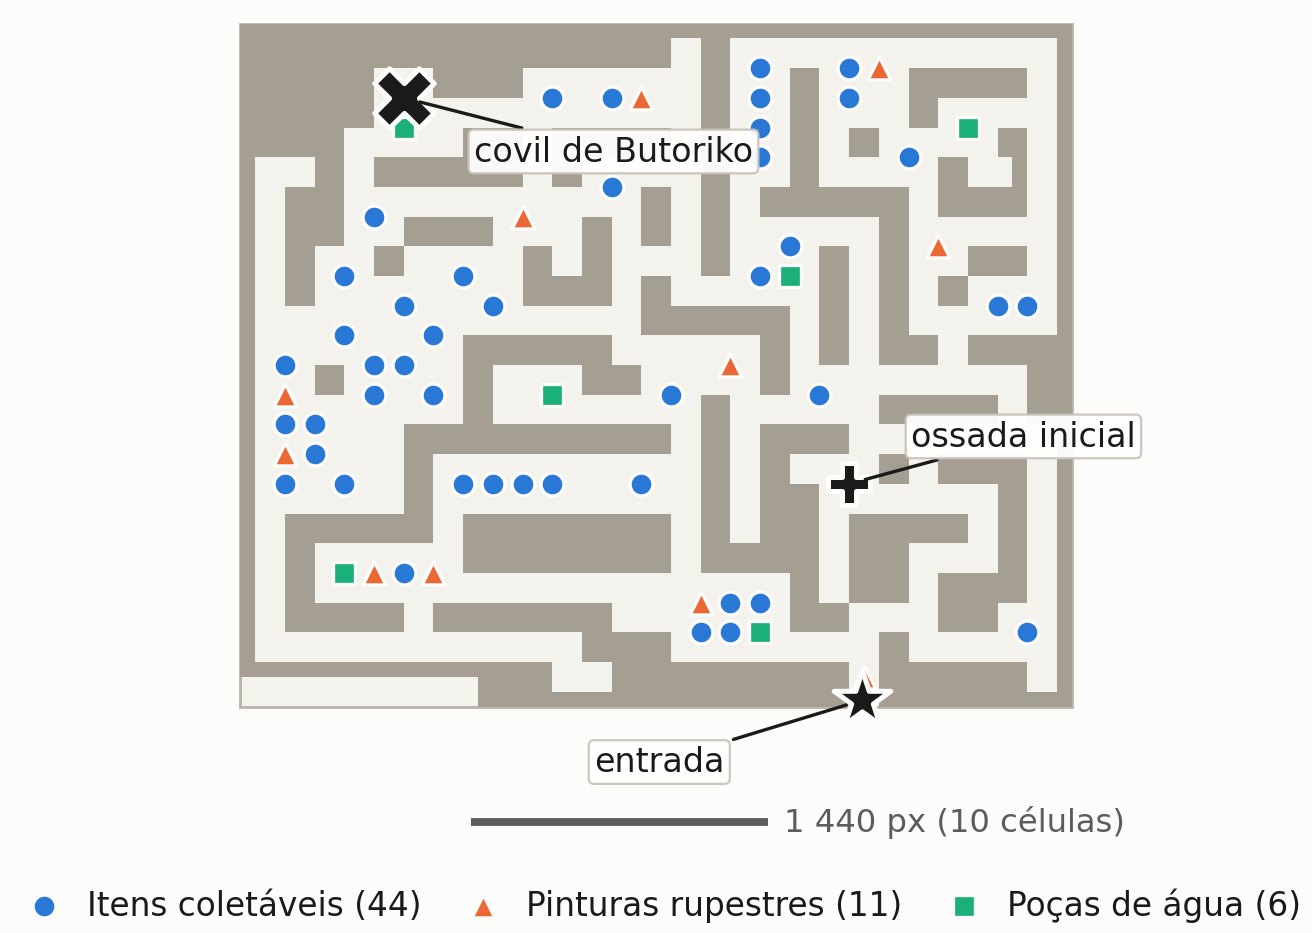
\includegraphics[width=\columnwidth]{planta_gruta.png}
\caption{Planta da gruta reconstruída a partir da geometria de colisão do
\textit{tileset} (544 polígonos de rocha sobre 636 células). A distribuição de itens é
mais densa no quadrante ocidental, oposto à entrada; o covil de Butoriko fica no extremo
noroeste. O labirinto não é gerado proceduralmente: resulta da combinação de dezesseis
variantes de \textit{tile} desenhadas à mão.}
\label{fig:planta}
\end{figure}

A distribuição espacial visível na figura não foi projetada como tal, mas emergiu do
posicionamento manual e revela uma propriedade útil: a densidade de itens cresce à
medida que o jogador se afasta da entrada, no canto inferior direito, em direção ao
covil, no extremo oposto. A recompensa e o perigo crescem juntos ao longo do mesmo eixo,
a propriedade que a literatura de \textit{roguelike} associa à decisão de
profundidade~\cite{cartlidge2024,toh2021}. Vale antecipar, porém, o que a
Seção~\ref{sec:resultados} mostra: sem saída implementada, esse gradiente não chega a
forçar decisão nenhuma. Ele descreve o jogo projetado, não o entregue. Onze pinturas
rupestres estão espalhadas pelo mapa, cinco delas duplicadas (``gêmeas'') em regiões
distantes, para que o jogador que entre por outro caminho ainda encontre a receita.

\begin{figure}[t]
\centering
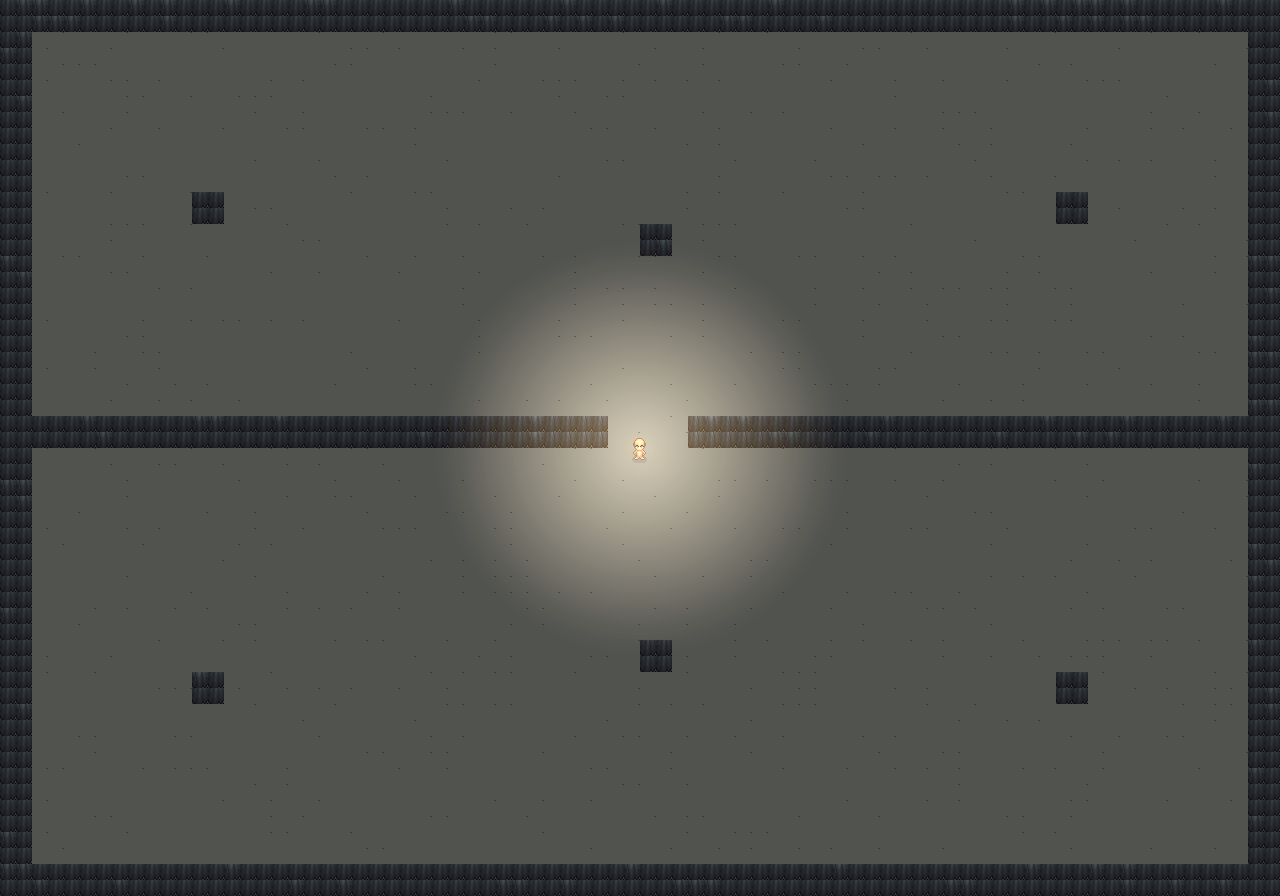
\includegraphics[width=\columnwidth]{tela_jogo.png}
\caption{Captura do protótipo, com gama corrigida para impressão. O halo da tocha é o
único campo visível; note que a luz para nas quinas de rocha em vez de contorná-las: é o efeito dos polígonos de oclusão do \textit{tileset}, e é o que faz a gruta se revelar por
linha de visada e não por raio.}
\label{fig:tela}
\end{figure}

\subsection{Itens, receitas e a matéria do mito}

O catálogo de itens é a parte do artefato em que a narrativa sobrevive de forma mais
direta. A Tabela~\ref{tab:itens} lista os treze itens e as cinco receitas.

\begin{table}[t]
\caption{Catálogo de itens e receitas de combinação}
\label{tab:itens}
\centering
\footnotesize
\begin{tabular}{p{2.6cm}p{1.05cm}p{3.5cm}}
\toprule
\textbf{Item} & \textbf{Peso} & \textbf{Efeito / composição} \\
\midrule
\multicolumn{3}{l}{\textit{Matéria-prima}} \\
Cipó & 1 & defesa 1; base de armadilhas \\
Raiz de unha-de-gato & 1 & cura 25 \\
Flor de crauá & 1 & fibra e seiva para veneno \\
Graveto de fogo & 1 & recarrega 20 s de tocha \\
Folhas secas & 1 & recarrega 10 s de tocha \\
Cuia & 2 & recipiente vazio \\
Pedrinhas & 1 & ataque 3, arremessável \\
Tronco de sucupira & 5 & ataque 10 \\
\midrule
\multicolumn{3}{l}{\textit{Compostos (aprendidos nas pinturas)}} \\
Cuia com água & 3 & cuia + folhas secas; cura 15 \\
Cuia com veneno & 3 & cuia com água + flor de crauá; ataque 12 \\
Pá & 3 & pedrinhas + graveto + cipó; ataque 8, defesa 2 \\
Armadilha de tronco & 4 & tronco de sucupira + cipó; dano 70 \\
Armadilha de espinhos & 3 & pá + folhas secas + flor de crauá; dano 45 \\
\bottomrule
\end{tabular}
\end{table}

Quatro dos oito itens de matéria-prima vêm diretamente da narrativa: o cipó, a raiz de
unha-de-gato, a flor de crauá (outra bromélia, como o coroatá citado no relato) e o
tronco de sucupira. No mito, esses elementos são obstáculos que o herói dispõe no
caminho de fuga; no jogo, são recursos que o jogador recolhe e combina. A transformação
é significativa e voltaremos a ela: o mito descreve preparação, o jogo implementa
coleta.

Duas propriedades do catálogo merecem nota porque não são explicadas em lugar nenhum do
projeto. A primeira: os pesos não se conservam na combinação: a armadilha de tronco pesa
4, contra 6 dos seus dois ingredientes, de modo que combinar alivia a carga. Isso faz da
bancada de mistura um incentivo mecânico, e não apenas narrativo, mas o efeito é
consequência de valores escolhidos item a item, e não de uma regra declarada. A segunda:
há dois caminhos para obter água. A receita ensinada nas pinturas produz cuia com água a
partir de cuia e folhas secas, enquanto as seis poças espalhadas pela gruta
(Fig.~\ref{fig:planta}) enchem diretamente uma cuia vazia. Os dois caminhos coexistem
sem que nada no jogo os relacione, resíduo de dois desenvolvedores resolvendo o mesmo
problema em eixos separados, e o exemplo mais concreto da especialização discutida na
Seção~\ref{sec:resultados}.

\subsection{Butoriko}

A serpente é implementada como agente autônomo com 628 linhas de GDScript, o segundo
maior \textit{script} do projeto. Vagueia pela gruta com mudanças de direção sorteadas a
intervalos de 0{,}8 a 2{,}5 segundos, evitando reversões imediatas, e sonda colisões
antes de virar. Detecta o jogador num raio de 180~px, com verificação de linha de visada
contra a camada de colisão das paredes, e passa a persegui-lo a 1{,}2 vez a velocidade
de vagueio. Emite um rosnado em intervalos aleatórios de 30 a 120 segundos, com
atenuação por distância até 800~px, recurso de tensão sonora que informa presença sem
informar posição. Deixa um rastro de marcas no chão, com intervalo e espaçamento
configuráveis. Tem 200 pontos de vida; quando é abatida, o jogo vai para a tela de
vitória.

%=======================================================================
\section{Resultados}
\label{sec:resultados}

\subsection{Correspondência entre mito e mecânica}

O primeiro resultado é a matriz da Tabela~\ref{tab:mito}, que registra, elemento a
elemento, o que da narrativa chegou ao artefato e sob que forma. Ela é apresentada aqui
como instrumento auditável: qualquer leitor pode confrontá-la com o repositório.

\begin{table*}[t]
\caption{Correspondência entre elementos da narrativa e mecânicas implementadas. Dos nove elementos, um chegou implementado ao protótipo, um parcialmente e sete não chegaram}
\label{tab:mito}
\centering
\footnotesize
\begin{tabular}{p{3.9cm}p{5.6cm}p{5.6cm}}
\toprule
\textbf{Elemento narrativo} & \textbf{Tradução projetada (SGDD)} & \textbf{Estado no protótipo} \\
\midrule
Butoriko devora os Boé e guarda os corpos na caverna &
Ossadas espalhadas pela gruta, com pertences das vítimas sobre elas &
\textbf{Implementado} como cenário e como ossada persistente de morte anterior; os itens não são caracterizados como pertences de vítimas \\[2pt]

A mãe de Pari Jura é levada; o colar fica na entrada &
Colar da mãe como objetivo narrativo visível no nível 1 e na tela final &
\textbf{Não implementado.} O gancho narrativo sobrevive apenas no texto de abertura \\[2pt]

Pari Jura treina antes de enfrentar a serpente &
Aldeia como \textit{hub} entre incursões: fôlego, força, vagas de carga &
\textbf{Não implementado.} Não há progressão entre tentativas \\[2pt]

Coroatá, cipó unha-de-gato, cipó urubamba e cerne de sucupira &
Quatro obstáculos plantáveis, com efeitos distintos (atrasar, ferir, emaranhar, prender) &
\textbf{Parcialmente implementado} como matéria-prima combinável em duas armadilhas (dano 70 e 45), e não como quatro obstáculos distintos \\[2pt]

O herói acorda o monstro de propósito &
Ruído como recurso: carga pesada, golpe em pedra, pedra atirada &
\textbf{Não implementado.} Butoriko detecta por raio e linha de visada, sem modelo de ruído \\[2pt]

A serpente só morre presa sob o cerne &
Butoriko imune ao cacete; vitória exige a armadilha correta no lugar correto &
\textbf{Não implementado.} Butoriko tem 200 pontos de vida e morre por dano acumulado de qualquer fonte \\[2pt]

A aldeia volta e cada um leva de volta a lembrança da sua vítima &
Tela final com a devolução das lembranças &
\textbf{Não implementado.} Tela de vitória genérica \\[2pt]

A gruta como morada das almas (\textit{aroe}) &
\textit{Aroe} nas ossadas, imitando os movimentos do jogador com atraso &
\textbf{Não implementado} \\[2pt]

Sair da gruta com o que se recolheu &
Extração: qualquer boca de gruta, com barra de três segundos; a incursão só conta se o jogador sai &
\textbf{Não implementado.} Existe o método \texttt{registrar\_saida()} em \texttt{Fase.gd} e o campo \texttt{ponto\_recomeco} em \texttt{GameState}, mas nenhuma saída está instanciada na cena \\
\bottomrule
\end{tabular}
\end{table*}

O padrão que a tabela revela é nítido, e não o esperávamos. O que sobreviveu à
implementação foi \textbf{matéria}: as plantas do mito viraram itens, a caverna virou
mapa, a serpente virou agente. O que não sobreviveu foi \textbf{estrutura}: a preparação
antes do confronto, o ruído como escolha, a condição de vitória que exige o plano, o
retorno à aldeia e, sobretudo, a extração.

Essa distinção importa porque, na leitura de Bogost~\cite{bogost2007} e
Madsen~\cite{madsen2017}, é exatamente a estrutura que carrega o argumento. A matéria é
representação; a estrutura é retórica procedural. Das nove linhas da
Tabela~\ref{tab:mito}, uma está implementada, uma parcialmente e sete não: o protótipo
entregue \emph{cita} o mito (nos nomes, nas plantas, no lugar) e praticamente não o
\textit{argumenta}.

\subsection{Distância entre o projetado e o implementado}

O segundo resultado quantifica essa distância. A Tabela~\ref{tab:gap} confronta a versão
consolidada do SGDD~\cite{sgdd2026} com o artefato entregue.

\begin{table}[t]
\caption{Documento de design \textit{versus} protótipo entregue}
\label{tab:gap}
\centering
\footnotesize
\begin{tabular}{p{2.35cm}p{2.5cm}p{2.5cm}}
\toprule
\textbf{Dimensão} & \textbf{SGDD} & \textbf{Protótipo} \\
\midrule
Estrutura & 3 níveis + aldeia & 1 nível \\
Geração do mapa & procedural a cada incursão & desenhada à mão \\
Duração da tocha & 90 s & 60 s \\
Obstáculos & 4 tipos distintos & 2 armadilhas \\
Condição de vitória & prender sob o cerne & reduzir 200 PV \\
Ruído & recurso gerenciável & ausente \\
\textit{Aroe} & inimigo com atraso & ausente \\
Extração & barra de 3 s em qualquer boca & ausente \\
Progressão & aldeia entre incursões & ausente \\
Criaturas menores & morcegos, aranhas, cobras & cena existe, sem instâncias \\
\midrule
Combinação de itens & receitas nas pinturas & \textbf{implementado} (5) \\
Peso e velocidade & carga retarda & \textbf{implementado} \\
Tocha dinâmica & luz encolhe & \textbf{implementado} \\
Perda por morte & 1 item por categoria & \textbf{implementado} \\
Ossada persistente & guarda o excedente & \textbf{implementado} \\
Chefe perseguidor & detecta e persegue & \textbf{implementado} \\
\bottomrule
\end{tabular}
\end{table}

Uma ausência merece nota à parte porque não é de sistema, e sim de conteúdo: a cena
\texttt{Enemy.tscn} está implementada, com perseguição, dano por contato e vagueio, mas
\emph{nenhuma criatura menor foi instanciada na gruta}. Há uma mensagem de \textit{commit} compatível com um corte deliberado, ``sem inimigos, ajustes nos textos'', embora ela sozinha não prove intenção. O efeito colateral é que, no protótipo entregue,
todo o risco da caverna se concentra em um único agente, o que enfraquece a tensão da
exploração longe do covil.

A leitura da tabela por categoria é o achado, com uma ressalva. Tudo o que foi
implementado é \textbf{local}: mecânicas que se resolvem dentro de uma cena, entre o
jogador e um objeto próximo: pegar, combinar, iluminar, apanhar, morrer. Entre o que
ficou de fora, os itens de maior peso são \textbf{globais}: a aldeia, a progressão entre
incursões e a extração exigem estado atravessando cenas ou sessões. A ressalva é que nem
todo corte é dessa natureza: a duração da tocha, o número de tipos de obstáculo, a
geração procedural do mapa e a condição de vitória condicional resolvem-se dentro de uma
única cena e ainda assim caíram. O que a tabela sustenta, portanto, não é que só o
global foi cortado, e sim que \emph{nenhum} sistema global sobreviveu, enquanto a
maioria dos locais sobreviveu.

Isso é consistente com o que Politowski \textit{et al.}~\cite{politowski2021} observam
sobre causas-raiz humanas e de processo, e admite uma explicação simples: mecânicas
locais podem ser desenvolvidas, testadas e integradas por uma pessoa em uma sessão de
trabalho; mecânicas globais exigem acordo prévio sobre representação de estado entre os
dois desenvolvedores, e esse acordo é caro num projeto de doze dias com trabalho
assíncrono. O \textit{autoload} \texttt{GameState} foi criado justamente para sustentar
esse estado global, e os vestígios do que se pretendia estão lá:
\texttt{ponto\_recomeco}, \texttt{tem\_recomeco}, \texttt{registrar\_saida()}. O
mecanismo foi codificado; o que faltou foi instanciar as saídas na cena e fechar o laço.

Registramos isso como a hipótese mais transferível do relato, hipótese e não lei, porque
um caso não a sustenta: em projetos curtos, o encolhimento de escopo pode não ser
aleatório nem proporcional, recaindo primeiro sobre os sistemas que atravessam
fronteiras de cena, ou seja, justamente sobre aqueles que carregam a estrutura da
experiência. Testá-la exigiria examinar outros relatos de projeto curto sob a mesma
grade.

\subsection{Processo de desenvolvimento}

O histórico do repositório registra 57 \textit{commits} distribuídos de forma fortemente
desigual ao longo da janela de doze dias: 48 deles, 84\%, ocorreram nos últimos três
dias. A divisão de trabalho entre os dois desenvolvedores foi equilibrada em volume e
nitidamente especializada em conteúdo: a leitura das mensagens de \textit{commit} mostra
um eixo de inventário, itens, combinação e interface e outro eixo de mundo,
\textit{tilemap}, oclusão, arte e animação, com poucos pontos de contato. Essa
especialização e a separação entre estado global e catálogo estático descrita na
Seção~\ref{sec:artefato} atuaram na mesma direção: juntas, mantiveram a árvore livre de
conflitos de mesclagem, ao preço de tornar caro fechar qualquer sistema que dependesse
dos dois eixos ao mesmo tempo, como a extração.

Vale registrar o custo desses três dias finais. Boa parte dos \textit{commits} finais
trata de ajustes de percepção e não de funcionalidade nova: escala do chefe, ordem de
desenho do herói sobre os itens, colisão, sprites armado e desarmado, animação de morte,
som de passos. Esse trabalho é frequentemente subestimado no planejamento, como observam
Washburn \textit{et al.}~\cite{washburn2016}, e é o que separa um protótipo que funciona
de um protótipo que se deixa jogar.

\subsection{Avaliação preliminar com jogadores}
\label{sec:playtest}

Uma sessão informal de teste foi conduzida ao final do desenvolvimento. Adotamos como
grade de análise o quadro de três dimensões de Camuñas-García
\textit{et al.}~\cite{camunas2023} (cognitiva, emocional e comportamental), que permite separar o que o jogador aprendeu, o que sentiu e o que fez.

\preencher{descrever o protocolo: quantos participantes, perfil (colegas de turma?
pessoas de fora?), se jogaram a build Windows ou a web, quanto tempo cada um jogou, se
houve observação direta ou relato posterior, se houve roteiro de perguntas}

A Tabela~\ref{tab:playtest} organiza os achados.

\begin{table}[t]
\caption{Achados do teste informal com jogadores}
\label{tab:playtest}
\centering
\footnotesize
\begin{tabular}{p{1.35cm}p{3.0cm}p{2.6cm}}
\toprule
\textbf{Dimensão} & \textbf{Achado} & \textbf{Resposta de projeto} \\
\midrule
Cognitiva
& \preencher{o jogador entendeu que as pinturas ensinam receitas? Encontrou a bancada de mistura? Percebeu a relação peso/velocidade?}
& \preencher{o que foi mudado, ou o que fica como trabalho futuro} \\[3pt]
Emocional
& \preencher{a escuridão e a tocha produziram tensão? O rosnado de Butoriko funcionou? Houve frustração com a perda de itens?}
& \preencher{} \\[3pt]
Comportamental
& \preencher{o jogador explorou ou correu para o fundo? Usou armadilhas ou enfrentou no cacete? Voltou para buscar a própria ossada?}
& \preencher{} \\[3pt]
Cultural
& \preencher{o jogador percebeu que os itens vêm de uma narrativa específica? Perguntou de onde vinha a história?}
& \preencher{} \\
\bottomrule
\end{tabular}
\end{table}

Duas hipóteses de projeto, derivadas do código e não da sessão, orientam a leitura dos
dados quando eles forem coletados. A primeira: sem a mecânica de extração, é plausível
que o custo da morte seja lido como punição arbitrária, e não como consequência de uma
decisão do jogador, porque a decisão de sair, que daria sentido ao risco, não existe no
protótipo. A literatura próxima é sugestiva, ainda que não decisiva: Tomé
\textit{et al.}~\cite{tome2020} mostram que a aversão à perda opera dentro do jogo, e West
\textit{et al.}~\cite{west2022} que a morte permanente pode aumentar a apreciação quando
mediada pelo luto. Nenhum dos dois testa a moderação por agência que a nossa hipótese
supõe, e é isso que o teste com jogadores precisaria verificar. A segunda: o modo de
teste embutido no jogo (\texttt{GameState.modo\_god}) foi criado no meio do
desenvolvimento e reduziu sensivelmente o custo de verificar regiões distantes do mapa,
pequena decisão de ferramental com retorno alto, do tipo que Petrillo \textit{et
al.}~\cite{petrillo2009} já apontavam como recorrentemente negligenciado.

\subsection{Aderência ao objetivo educacional}

O artefato foi projetado para veicular elementos culturais, e é honesto medir quanto
disso ele efetivamente veicula. Uma sessão completa expõe o jogador a: o topônimo Aroe
Jari e o nome do herói Pari Jura; quatro espécies vegetais do cerrado com uso
tradicional descrito na ficha de cada item; o nome Butoriko; e uma estrutura narrativa
de perda e vingança apresentada em uma única linha de texto na abertura. Até a versão descrita nas
subseções anteriores, isso era tudo: o jogo não expunha o nome Boé, o contexto geográfico
de Mato Grosso, o conceito de \textit{aroe} que dá nome à gruta, nem qualquer indicação de
que os Boé existem hoje e vivem em terras indígenas
específicas~\cite{serpa2025,ibge2025}.

Uma tela de contexto, acessível do menu e da tela de vitória, foi acrescentada ao
protótipo em resposta a esse diagnóstico. Ela atribui a história à tradição Boé, credita a
adaptação à equipe, nomeia o povo, situa as terras indígenas de Meruri, Sangradouro,
Tadarimana e Perigara, explica o que é \textit{bakaru} segundo Souza~\cite{souzabakaru} e
lista as leituras que informaram o projeto, incluindo o trabalho de
Ekureu~\cite{ekureu2025}. Uma linha na tela inicial e na tela de vitória antecipa o
essencial, porque uma tela atrás de botão é uma tela que a maior parte dos jogadores não
abre.

O que permanece pendente é a segunda metade da correção: as fichas de item continuam
descrevendo apenas a função mecânica de cada planta, quando poderiam dizer o que ela é
fora do jogo. É ali que a coleta viraria contato, sem custo de mais uma tela. À luz da
Lei~11.645/2008~\cite{brasil2008}, essa diferença não é ornamental: Moreira e
Barragán~\cite{moreira2025} argumentam que jogos de matriz indígena só operam
pedagogicamente quando o vínculo com o povo de origem é explicitado, e o vínculo agora
existe, mas ainda concentrado num só lugar do jogo.

%=======================================================================
\section{Discussão}
\label{sec:discussao}

\subsection{Extração sobre cosmologia: a objeção de Arrivabene}

A objeção mais séria ao desenho do jogo é a de Arrivabene~\cite{arrivabene2025} e
Byrd~\cite{byrd2025}: as convenções correntes de game design carregam pressupostos
coloniais, e o extrativismo (entrar num território, retirar valor, sair) é o mais
evidente deles. Kinder~\cite{kinder2021} mostra, analisando \textit{Thunderbird Strike},
que um jogo indígena pode fazer o movimento contrário e tomar o próprio extrativismo
como objeto de crítica jogável, o que estabelece que a escolha do gênero não é destino.
Construir um jogo de \textit{extração} sobre uma cosmologia indígena, numa caverna que a
tradição associa à morada das almas, é, no mínimo, uma escolha que precisa ser
defendida.

Há uma defesa disponível e ela não é trivial. Na narrativa, o
que o herói retira da caverna não é riqueza, é \textit{a lembrança dos mortos}: no fim,
a aldeia inteira volta e cada representante leva de volta um objeto da sua vítima. Se a
mecânica de extração tivesse sido implementada com esse conteúdo (carregar os pertences
dos devorados de volta para fora, com o peso e o risco que isso impõe), a ``extração''
estaria invertida em relação ao seu sentido colonial: não retirar valor de um
território, mas devolver os mortos aos vivos. Essa é, no nosso entendimento, a leitura
mais forte que o projeto poderia sustentar, e é a razão pela qual a ausência da extração
no protótipo é mais grave do que a de qualquer outro sistema.

O protótipo entregue não sustenta essa defesa. Nele, os itens são recursos genéricos,
descritos por peso, ataque e defesa; não são lembranças de ninguém. O jogo argumenta,
proceduralmente, que uma caverna é um lugar de onde se tiram coisas úteis. É exatamente
o que Arrivabene descreve. Registramos isso não como autocrítica de praxe, mas como
resultado: mostra que a distância entre reinscrever e inverter uma lógica colonial pode
ser tão pequena quanto um campo no catálogo de itens e uma mecânica de saída.

Vale precisar de onde vem essa defesa, porque o crédito importa. O
elemento em que a inversão se apoia, o retorno da aldeia para recolher as lembranças dos
mortos, está na narrativa da tradição Boé, e não é invenção nossa. Nosso é apenas o
reconhecimento de que ele resolveria um problema de design: quando o objeto da extração
deixa de ser riqueza e passa a ser a memória dos mortos, o laço inverte o sentido colonial
que Arrivabene~\cite{arrivabene2025} atribui ao gênero. A ideia é deles; a leitura em
chave de mecânica é nossa.

\subsection{Onde este projeto está na escala de soberania}

Aplicando o critério de LaPensée \textit{et al.}~\cite{lapensee2022}, este projeto não
está em posição soberana nem em codesenvolvimento. Está abaixo do patamar consultivo,
porque não houve consulta. A Tabela~\ref{tab:protocolo} propõe um quadro de decisão
rastreável, não como certificado de boa conduta, mas como instrumento de registro: para
cada decisão sensível, o que foi feito, com que fundamento, e o que precisaria acontecer
para elevar o projeto de patamar.

\begin{table}[t]
\caption{Quadro de decisão rastreável para representação cultural}
\label{tab:protocolo}
\centering
\footnotesize
\begin{tabular}{p{1.9cm}p{2.6cm}p{2.8cm}}
\toprule
\textbf{Decisão} & \textbf{O que foi feito} & \textbf{O que falta} \\
\midrule
Origem da narrativa
& Declarada como da tradição Boé; adaptação creditada à equipe; referência documental não localizada (Seç.~\ref{sec:referencia})
& Conferir o v.~II da \textit{Enciclopédia Bororo} e citar quando possível \\[3pt]
Consulta à comunidade
& Nenhuma
& Contato com associações Boé (Meruri, Tadarimana) antes de qualquer distribuição pública \\[3pt]
Material ritual
& Nenhum grafismo clânico nem elemento cerimonial reproduzido; ossadas e a associação da gruta com os mortos são, porém, conteúdo funerário
& Submeter nomes, grafismos e trilha a revisão de interlocutores Boé \\[3pt]
Grafismos e arte
& Pinturas rupestres inventadas, não reproduzidas de sítio real
& Dizer isso na tela de contexto, hoje implícito \\[3pt]
Língua
& Apenas dois nomes próprios; nenhum texto em Boé
& Se houver uso da língua, revisão por falante \\[3pt]
Repartição de benefícios
& Não aplicável (sem receita); código sob licença aberta
& Definir antes de qualquer versão comercial \\[3pt]
Nomeação do povo
& O artigo usa ``Boé''; o jogo não nomeia o povo
& Nomear no jogo, com contexto \\
\bottomrule
\end{tabular}
\end{table}

O valor desse quadro não está em nenhuma linha isolada, e sim no fato de que a coluna da
direita é acionável. Ele transforma princípios (CARE~\cite{carroll2020},
Convenção~169~\cite{oit1989} e soberania~\cite{lapensee2022}) em uma lista de pendências
que uma equipe pequena consegue de fato executar, que é precisamente a carência que
Laiti~\cite{laiti2025} e Costa \textit{et al.}~\cite{costa2025} apontam na literatura.

\subsection{Aplicando a regra ao próprio artefato}
\label{sec:autoaplicacao}

Uma regra que os autores enunciam e não aplicam a si mesmos não é uma contribuição, é
retórica. Como a subseção anterior sustenta que a declaração de estatuto precisa estar no
artefato, e não apenas no artigo, cabe medir o projeto pelo próprio critério, em três
lugares.

No repositório: a declaração da Seção~\ref{sec:procedencia} foi incorporada ao
\texttt{README}, de modo que ninguém encontre o código sem encontrar o estatuto do
material. Na circulação: o jogo não é publicado em loja nem divulgado como jogo sobre a
cultura Boé, e o repositório é material de pesquisa que acompanha este artigo.

E, agora, dentro do jogo, que é onde mais importa e onde o projeto falhava. Até a versão
anterior, o jogador saía da sessão sem saber que a história vinha da tradição de um povo
que existe hoje, e sem saber quais partes daquilo eram invenção dos desenvolvedores. A
tela descrita na Seção~\ref{sec:resultados} declara as duas coisas, e uma decisão de
projeto merece ser explicitada aqui: a declaração é \emph{não-diegética}, isto é, fala na
voz dos autores e não na voz do jogo. Uma declaração de autoria colocada dentro da ficção,
numa pintura rupestre por exemplo, não declararia nada, porque viraria fala dos antigos. O
conteúdo cultural pode ser diegético; a atribuição, não.

\subsection{Usar sem poder citar}

A Seção~\ref{sec:referencia} descreve uma situação que a literatura de patrimônio
imaterial discute pouco e que a prática encontra o tempo todo: o material é real, a
comunidade o transmite, e não existe registro publicado que permita citá-lo. A norma
acadêmica não tem casa para isso. Ela pressupõe que o que não se cita não se usa, o que,
aplicado ao patrimônio imaterial, produz um resultado perverso: exclui do trabalho
acadêmico justamente o que é mais imaterial.

As duas saídas correntes são ruins. Abandonar o material significa aceitar que só o
patrimônio já digitalizado pode ser estudado, o que reproduz, na bibliografia, a mesma
assimetria de acervo que a digitalização criou. Usar sem dizer nada é a saída que se
pratica em silêncio, e é a que alimenta a circulação de versões sem procedência que a
literatura sobre representação indígena documenta há
décadas~\cite{wallis2023,martinsneto2024}.

A terceira saída, que adotamos, é declarar a cadeia inteira: de onde o material veio, o
que foi buscado, o que não foi encontrado, o que falta conferir, e onde termina a tradição
e começa a adaptação. Isso não substitui a referência, e não pretende substituir. Faz duas
coisas mais modestas: permite que o leitor julgue o material pelo que ele é, e deixa a
pendência visível, em vez de resolvida por omissão. Uma exigência acompanha a saída, e é a
que costuma ser esquecida: a declaração precisa estar no artefato, e não apenas no artigo
que fala sobre ele, porque quem joga não lê o artigo.

\subsection{Limitações}

Cinco limitações circunscrevem o alcance do que foi dito. Primeira e mais importante: não
conseguimos estabelecer a referência documental da narrativa, de modo que a
Tabela~\ref{tab:mito} compara o jogo com a versão que chegou ao projeto, e não com um
registro conferido; ela vale como método de auditoria da adaptação, não como prova de
fidelidade à tradição. Segunda: não houve consulta à comunidade
Boé, o que exclui o trabalho do patamar de codesenvolvimento e limita o que ele pode
reivindicar sobre representação. Terceira: a avaliação com jogadores é informal, de
amostra pequena e sem instrumento validado, servindo para orientar projeto e não para
sustentar inferência. Quarta: os autores do artigo são os desenvolvedores do artefato, e
a análise de escopo é autorrelato, mitigado mas não eliminado pela ancoragem em
evidência de repositório. Quinta: a comparação entre design e implementação usa a
segunda versão do SGDD como referência, embora o projeto tenha sido iniciado sob a
primeira, o que pode superestimar a distância entre o projetado e o entregue.

%=======================================================================
\section{Conclusão e trabalhos futuros}
\label{sec:conclusao}

Este artigo relatou o projeto, o desenvolvimento e a avaliação preliminar de
\textit{Grutas de Aroe-Jari}, jogo digital 2D construído em Godot~4 sobre uma narrativa
atribuída ao povo Boé (Bororo). O artefato reúne 3.851 linhas de GDScript, dezesseis cenas,
uma gruta de 636 células com 544 polígonos de rocha, treze itens distintos em 44
instâncias, cinco receitas ensinadas por pinturas rupestres diegéticas e um chefe
perseguidor, produzidos por dois desenvolvedores em doze dias.

Três resultados principais foram reportados. A matriz de correspondência mito--mecânica
mostrou que o que sobreviveu à implementação foi a matéria da narrativa (plantas,
caverna, serpente) e não a sua estrutura: a preparação, o ruído como escolha, a condição
de vitória condicional e a extração ficaram de fora. A comparação entre o documento de
design e o artefato localizou o encolhimento de escopo de forma sistemática nos sistemas
que atravessam fronteiras de cena, e não uniformemente, o que constitui um alerta de
planejamento transferível a outros projetos curtos. E o relato da busca por um registro
publicado da narrativa, transmitida pela tradição Boé e ausente de todo acervo
digitalizado que alcançamos, sustentou o argumento sobre o descompasso entre tradição e
registro citável, e a proposta de declarar a cadeia inteira quando a referência não pode
ser estabelecida.

A continuidade está organizada em cinco frentes, em ordem de precedência. A primeira é o
contato com associações Boé, condição para qualquer elevação de patamar na escala de
soberania~\cite{lapensee2022}, e ocasião para submeter a eles a pergunta que nenhuma busca
bibliográfica responde: se reconhecem, nas referências que usamos, um uso que lhes pareça
adequado. A conferência documental do volume~II da \textit{Enciclopédia
Bororo}~\cite{albisetti1969} acompanha essa frente, para descartar coincidência com alguma
variante local ainda não digitalizada. A segunda é a implementação da extração
(instanciar as saídas, fechar o laço já parcialmente codificado em \texttt{GameState} e
substituir os itens genéricos pelas lembranças das vítimas), que é simultaneamente a
mecânica ausente mais importante e a única forma de sustentar a inversão do sentido
extrativista discutida na Seção~\ref{sec:discussao}. A quarta é uma avaliação com
instrumento validado, seguindo o quadro de três dimensões de Camuñas-García
\textit{et al.}~\cite{camunas2023} e o precedente de Emmons e
LaPensée~\cite{emmons2021}. A quinta é completar, nas fichas de item, o
contexto que a tela de contexto passou a dar em um só lugar: é ali, na coleta, que o
vínculo com o povo de origem deixaria de depender de o jogador abrir um menu.

\section*{Disponibilidade de artefatos}

O código-fonte, os documentos de design, os \textit{assets} e as \textit{builds} para
Windows e navegador estão disponíveis no repositório do projeto~\cite{repo2026}, que
carrega, no \texttt{README}, a declaração de origem da narrativa discutida nas
Seções~\ref{sec:procedencia} e~\ref{sec:autoaplicacao}. Todos os números apresentados neste artigo
foram extraídos programaticamente desse repositório e podem ser reproduzidos a partir
dele.

\section*{Agradecimentos}

Ao professor da disciplina CPS837 (Projeto de Jogos), do PESC/COPPE/UFRJ, pela
orientação ao longo do semestre. \preencher{confirmar o nome do professor e incluir
demais agradecimentos}

\bibliographystyle{IEEEtran}
\bibliography{references}

\end{document}
